\section{Snell波与斜坐标}
\label{sec:5.3}

倾斜叠加与Snell波紧密有关,但事情还不仅止于此,三种不同类型的道集(共炮点道
集,共检波点道集及共中心点道集)都可以作倾斜叠加,而在每种情形下其意义却均不相
同。

一个Snell波可以用普通反射数据进行倾斜叠加的办法把它合成出来,凡Snell波都可按
波动传播理论加以描述,尽管有横向速度变动、多次反射、横波等复杂性或者所有这些复杂
情形同时存在,你仍可望能够写出一个真实描述Snell波的波动方程。与此形成对照的是
CDP叠加,在这里,向下延拓就已经是一种近似了,即使在速度为常数时也是如此。我们当
然总可以返回炮点检波点空间内去作数据分析,但倾斜叠加是一种叠加处理,因而那就意味
着已经作过干扰处理和数据压缩了。

\subsection{野外资料中的Snell波信息}
\label{sec:5.3.1}

根据叠加原理,我们能由具有一切频率之正弦波的叠加形成一个脉冲函数,推广至三维
情形,沿所有方向传播之平面波叠加起来则形成一个点震源。与此相似,一个平面波可以是由
许多惠更斯二次点源叠加所成的结果,对勘探中所记录的点震源数据采取一种称为倾斜叠加
的适当叠加处理,则可以模拟Snell波。

假想一条地震测线内的所有炮点都在同一时间起爆,这时的下行波将近似为平面波(假
设我们忽略真实世界是三维而不是二维这个现实),由这样一种排列所记录到的资料完全可
以根谄常规资料模拟出来,只须将数据场遍及所有炮点坐标s求和即可\footnote{
设野外记录为户$(s, g,t)$,
其中,s为炮点坐标,g为检波点坐标,t为时间。取共检波点道集$p(s_1, g,
t)$, $p(s_2,g,t)$,......,不经动校正而全部直接叠加、因反射波时距曲线在检波点g附近的曲率较平缓,故为同相叠加而加
强,远离该点则因非同相干涉而减弱,因此得出$(g,t)$
空间内的近似上行平面波。如取共炮点道集$p(s, g_1, t)$、$p(s,
g_2,t)$,......作相同叠加处理,则得$(s,t)$空间内的近似下行平面波。---译者
},每个共
检波点道集内的各记录道要不经正常时差校正就求和。

要想模拟某种非垂直方向传播的Snell波,则必须按照所需描述的某个射线参量值$p_s=
dt/ds$使相继的激发保持一定的时间延迟,犹如是从水平飞行的超音速飞机所辐射出来的一
般。

如果是沿检波点坐标轴g而不是沿炮点坐标轴s将数据求和,情形会如何?这时所得结果
相当于业已准确调谐至只接收垂向传播之波的接收天线所记录的点源试验\footnote{
这段的意思是说:共炮点道集不经正常时差校正而直接叠加求和所得相当于炮点坐标空间$(s,t)$内的自激自收下行平面波。 ---译者
},在叠加求和之
前使检波点上的到达时间有时移,则可模拟只记录某一种Snell波的接收天线,比方说,记录
到参量为$p_g=dt/dg$、上行角度为$\sin\theta=p_gv$的波。

沿某一坐标轴进行积分就是沿某一坐标轴进行低通滤波的一种极端情形,介于点震源情
形和平面波情形这两种极端之间的是定向发射与接收的情形。

简单的传播过程使点源扰动散布至一定距离之处,波就似乎是有些像平面波或Snell波
了,这样就可以把波至显得几乎是呈平面形状之处的一小段同相轴当作Snell波进行分析。

总而言之,在炮点空间$(s,t)$内进行倾角滤波所得到的是下行Snell波,而在检波点
空间$(g,t)$内进行倾角滤波所得到的则是上行Snell波。


\subsection{噪音抑制与数据记录}
\label{sec:5.3.2}

噪音抑制(muting)的基本目的是消除水平传播的能量\footnote{
muting是常规地震处理中的一科预处理程序,又可译为切除处理,目的在于切除直达波和面波干扰,即所谓的水
平传播的能量。---译者
},这类能量与地层映象毫无关
系。典型的实现抑制切除之方法如\ref{sec:3.5}节所述,那就是说,采用某种加权函数将普遍超出炮
检距与时间之比值$(g-s)/t$某个门限值的数据均置零。噪音抑制处理可以切除许多水平传播
能量是没疑问的,但是要消除的还不仅限于此。因反向散射之故,常常在噪音抑制区之内还可
发现水平传播的能量,除掉它的办法必须采用倾角滤波而不是采用某种加权函数。在现代高
密度多道记录系统采用以前,低速传播的噪音往往在检波器电缆长度范围内形成空间假频现
象,以致进行倾角滤波行不通.如果出射角并非足够接近于垂直,就是说,如果$dt/dg$不是
足够小,这时波就可能不是来自勘探目的层。在炮点空间$(s,t)$内应用滤波不像在检波点
空间$(g,t)$内那么容易,因为在炮点空间内极少能非常稠密地记录数据。千万别跌入圈
套,认为可以对共中心点道集进行这种倾角滤波,反向散射的地滚波在共中心点道集内是没
有正常时差的(见\ref{sec:3.2}节)!

海水层底部散射往往很强,使得很难采用常规处理方法压制它。在\ref{sec:3.2}节中,我们已了
解其原因在于点溫散射意味着有双曲线型波至,它具有陡倾角,其到达时间一般比水层底部
反射时间要晚,因而会误认为它们具有沉积地层的叠加速度而不是水层速度。这时所需要的
是作两种倾角滤波,一种是抑制以非垂直角度离开各炮点的波,另一种则是抑制以非垂直角
度到达各检波点的波。现今的野外组合其滤波作用系以空间频率$k_x$为基础,如记录设备采用倾
角$(k/\omega)$的滤波而不是采用空间频率的滤波,资料中将会留有更多高频能量。\ref{sec:2.5}节中所
述具有时间因果性的递归倾角滤波在这里可能会起很好的作用。


\subsection{Snell波的合成}
\label{sec:5.3.3}

设我们用野外数据人工合成了一个下行的Snell波,然后设想一下上行波将会显得如何,
以及它将如何把有关地下界面的信息带给我们。

进行倾斜叠加要取测线上的数据$P(s,g,t)$,它是炮点位置s、检波器位置g和旅行时
间t的一个函数。然后,要在炮点遍及的范围内求和,从而合成作出犹如应当是由下行Snell波
发生了反射才能被记录到的上行波$U(g,t)$。即使可能存在有速度横向变化和多次反射,
情形仍应如此,不受影响。

因为涉及到三种不同类型的时间,求和过程有点混乱:
t=点震源野外记录内的时间。\\
$t'=t-p(g-s)$=解释时间。仅在$t'=0$之后才看得见最浅的反射面。\\
$t_{pseudo}$=具有移动震源之Snell假想排列记录内的时间。\\

在水平成层地层情形下,假想排列记录内的时间$t_{pseudo}$具有特定的特征:你将检波点坐标
移出越远,回声反射就会到达越晚。根据下列关系可从野外排列记录的时间t直接变换为解释时间t':
\begin{equation}
t'=t_{pseudo}-px=t-p(g-s)
\label{eq:ex5.3.1}
\end{equation}
图\ref{fig:slnt/snellwave}示意绘出了下行Snell波的情形。

\begin{figure}[H]
\centering
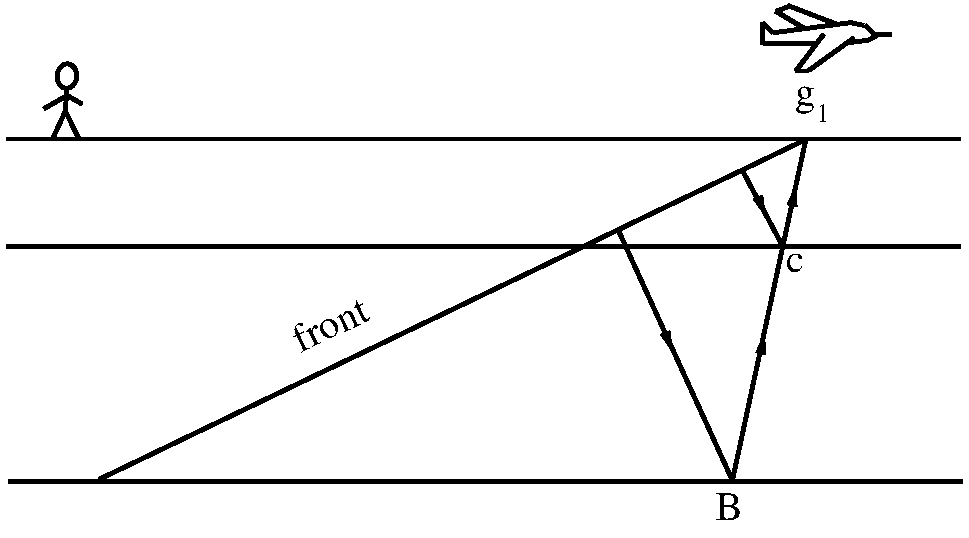
\includegraphics[width=0.65\textwidth]{slnt/snellwave}
\caption[snellwave]{Snell波的波阵面由两个地层反射,携带信息
上行返回至检波器$g_1$
}
\label{fig:slnt/snellwave}
\end{figure}

图\ref{fig:slnt/cspss}所示是一种假设的共检
波点道集,将该道集求和可模拟出图
\ref{fig:slnt/snellwave}中所见到的位于$g_1$上之Snell波。在图\ref{fig:slnt/snellwave}
中的由C点至B点的横向偏离距离与图\ref{fig:slnt/cspss}中相应的距离(图\ref{fig:slnt/cspss}中的两
个位置上)是完全相等的。对所有的检波点
重复进行上述沿炮点坐标的求和过程,即可由下行Snell波作出合成上行波。

\begin{figure}[H]
\centering
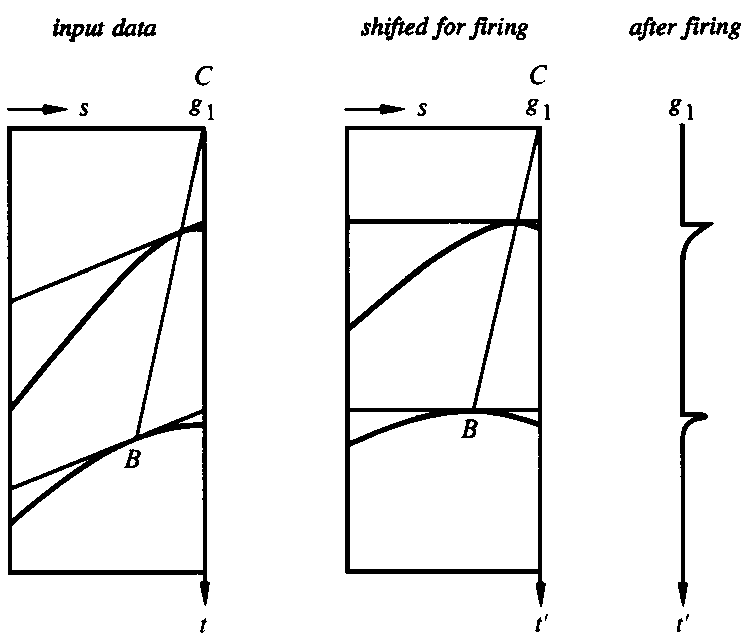
\includegraphics[width=0.65\textwidth]{slnt/cspss}
\caption[cspss]{左图是两个平反射界面情形下的位于
检波点$g_1$上的共检波点道集。中图表示,为准备用遍及炮点
坐标s进行求和而产生合成Snell波,数据已根据线性时差校正作
了时移。右图所示是检波点$g_1$上所记录到的Snell波记录道。
Snell波的地震剖面由许多像$g_1$的记录道并列组成。
}
\label{fig:slnt/cspss}
\end{figure}

% \subsection{根据倾斜叠加估计层速度}
% \label{sec:5.2.4}

% \ref{sec:1.5}节曾指出,向下延拓Snell波纯粹是个时移问题,时移量只与波的传播角度有关。例
% 如,关于时移的频率域方程就是
% \begin{equation}
% P(\omega,p,z_2)=P(\omega,p,z_1)e^{-i\frac{\omega}{r}\sqrt{1-p^2r^2}(z_2-z_1)}
% \label{eq:ex5.2.5}
% \end{equation}
% 向下延拓至第一个反射面时,我们发现第一个反射应在零时间到达。在偏移方法中,习惯的
% 作法是就零倾角射线来完成时间延迟,因此,延迟时间形式的向下延拓会展平第一个反射而
% 不改变零倾角射线。对数据进行时移使之在第一层的反射上排齐校直的过程,可用图\ref{fig:slnt/schultz}
% 中的第三个图形解释说明。该图的第一个图形表示速度模型,第二个图形表示地面上倾斜叠
% 加的结果。把第一个反射面按时间排齐校直之后,我们就得到了在第一层底部应被观测到的
% 数据。现在,次深曲线的是一个严格的椭圆,根据该次深的椭圆估计出次深层的速度。对所
% 有的深度将这种处理过程继续下去,直至处理完。这种速度估计方法是由P.Schultz
% ( 1982 ) 提出并试验过的。

% \begin{figure}[H]
% \centering
% 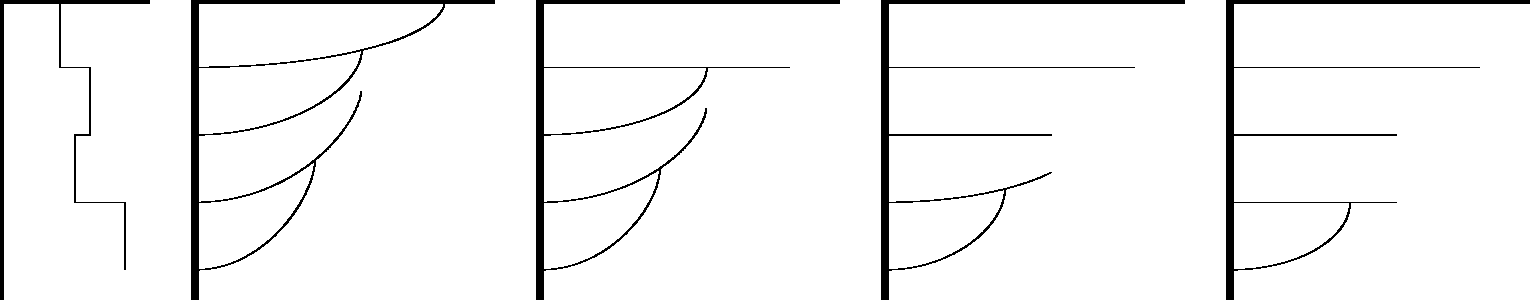
\includegraphics[width=0.65\textwidth]{slnt/schultz}
% \caption[schultz]{Schultz的相继各层展平方法}
% \label{fig:slnt/schultz}
% \end{figure}

% 图\ref{fig:slnt/schultz}还解释说明了由浅层高速层引起的困难。任何较深部低速层的反射给出的是一
% 种不完全的椭圆,它与上面的椭圆不相联,因为它看来要延伸超出该范围。较大的p值
% (图中的点状线)会丢失,因为它们被上面的高速层(低值)所阻塞限制。p的截止出现在
% 高速层的波趋于水平传播之处,所以,在较深的低速层底部不存在首波。

% Schultz根据某个橢圆作速度沽计的方法所进行的方式是:沿各种不同速度的扫描椭圆
% 进行求和,然后选出具有最强叠加效果的一个速度。因此,他的方法应当不受浅层高速层的
% 干扰。注意下列一点是有益的,在速度随深度而连续增大的时候,速度与深度的关系曲线可
% 以直接从图\ref{fig:slnt/schultz}最右端的图形读出来,速度与深度的关系曲线将是联接反射各端点(极
% 大值)的线,亦即联接各首波的那条线。

% \subsection{根据首波估计界面速度}
% \label{sec:5.2.5}

% 根据首波确定地层速度是地震学中的一个古老问题了
% 。在有可能的地方根据首波测定速
% 度是指在特定的深度上进行测定---分界面深度---所以,它具有甚至比层速度(两个反射
% 之间的深度间隔上的速度)还要好的深度分辨能力。

% 按传统的作法,首波速度分析涉及到识别追踪旅行时间。旅行时间很难在受干扰资料中
% 识別出来。Clayton与McMechan (1981)曾介绍过一种建立在波场本身基础上的、而不是
% 在追踪旅行时间基础上的新方法,他们解决首波速度分析问题就同波动方程偏移解决反射问
% 题一样。

% 与那类从剖面上的反向散射首波获取速度信息(见\ref{sec:3.5}节)的方法相同的思想,可以应
% 用于共中心点道集中的普通首波。在道集中,你可得到在向下延拓将能量聚焦到零炮检距的剖
% 面上所没有的额外信息。聚焦点可不是一个平凡的毫无特色的点。取一段没有反射而仅由一
% 个首波所组成的原始数据,向下延拓后在零炮检距上产生一聚焦点,该聚焦点是把具有和原
% 始未聚焦首波一样的时差$dt/dh$之零散能量集中起来而得到的结果。按所有可能的取向将各
% 聚集点相加起来(倾斜叠加),
% 从而把数据$u(h,\tau)$变换至倾角空间、比方说变换为$\bar{u}(p,\tau)$。在$(p,\tau)$
% 平面上地震能量已经集中的地方求出旅行时间深度$\tau$处地层的速度,该速度可
% 直接由$v(\tau)=1/p(\tau)$得出。已知$v(\tau)$,很容易就能求出$v(z)$。或者,整个计算过程也可以直接
% 按深度z来实现而不按旅行时间深度$\tau$来完成。

% Clayton与McMechan实际
% 是按相反的顺序来完成向下延拓和倾斜叠加的,他们首先是倾斜
% 叠加,然后再向下延拓的。在原理上,这些赴理过程不论按什么
% 顺序完成都行。要记住,我们是否成功是脱离不开正确的地层速
% 度的,进行倾斜叠加倒是不必
% 依靠地层速度,但是向下延拓却得依靠正确
% 速度。倾斜叠加仅需实现一次,如果它是首先
% 作的话。这就是为什么Clayton和McMechan按那种顺序方式作它的原因。图5.
% 2-5和图5.2 -6所示是他们的实例之一。

% 将Clayton与McMechan的方法同Schultz的方法比较一下。Schultz是用一种对椭
% 圆较大p值部分很敏感的方法将反射展平,
% Clayton与McMechan则只着眼于椭圆的最大
% p值部分。Schultz方法的好处是:一种以反射为
% 基础的方法是不受高速层干扰时,但是缺点是
% 要求在向下进行处理之际就得作出判断决定。
% Clayton与MeMechan则是把一个信息平面提
% 供给解释者,由解释者从这个平面中去选择速度。Clayton与MaMechan的速度空间是数据
% 的一个线性可逆函数,\ref{sec:5.4}节将要阐述从反射数据(不是首波)至速度空间的线性可逆变换。

% \begin{figure}[H]
% \centering
% 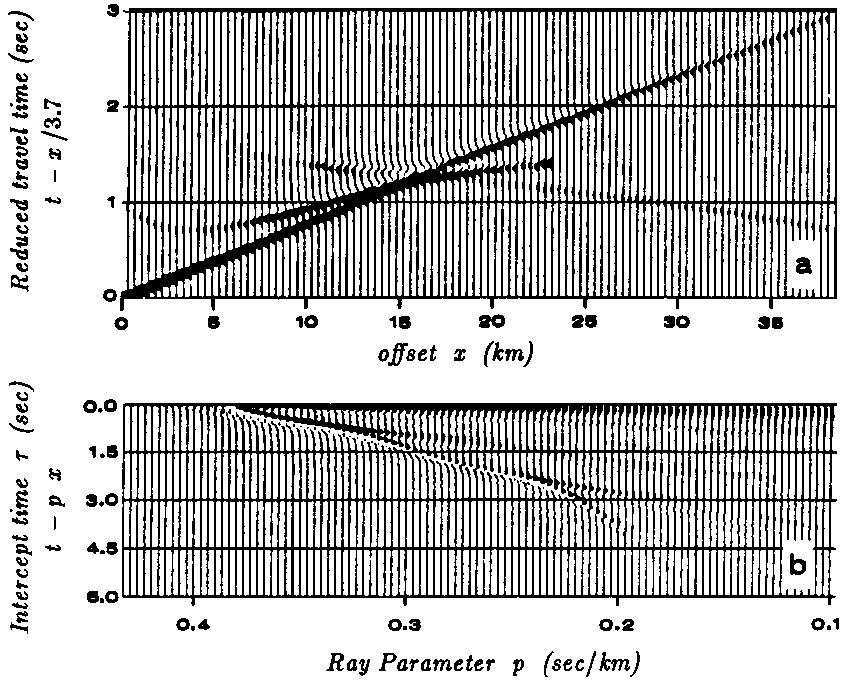
\includegraphics[width=0.65\textwidth]{slnt/sshead}
% \caption[sshead]{上图(a)是包含有一合成首波的剖面(以线性时差校正方式显示)
% 利用倾斜叠加将数据变换如图(b)的下半部分所示。这个已经过倾斜叠加的波场(b)的向下
% 延拓结果如图\ref{fig:slnt/sshead2}所示(Clayton与McMechan)}
% \label{fig:slnt/sshead}
% \end{figure}

% \begin{figure}[H]
% \centering
% 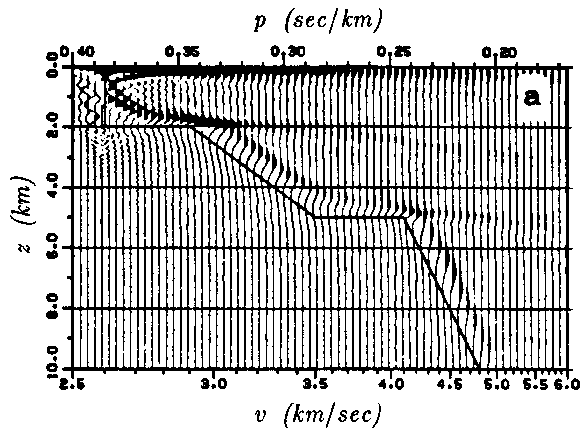
\includegraphics[width=0.65\textwidth]{slnt/sshead2}
% \caption[sshead2]{以正确的速度与深度关系函数(图中实线)对图\ref{fig:slnt/sshead}(b)
% 中的倾斜叠加波场进行向下延拓的结果}
% \label{fig:slnt/sshead2}
% \end{figure}

% \subsection{倾斜叠加与Fourier变换}
% \label{sec:5.2.6}

% 设$u(x,t)$为波场。在数学上,波场的倾斜叠加$\bar{u}(p,\tau)$被定义为:
% \begin{equation}
% \bar{u}(p,\tau)=\int u(x,\tau+px)dx
% \label{eq:ex5.2.6}
% \end{equation}
% 式\ref{eq:ex5.2.6}中,按x进行的积分是在$\tau$值恒定时完成的,积分路程就是$(x,t)$平面内的某条
% 倾斜直线。

% 在Fourier空间内很容易表示倾斜叠加。波场$u(x,
% t)$的二维Fourier变换之定义为:
% \begin{equation}
% U(k,\omega)=\\int e^{i\omega t-ikx}u(x,t)dxdt
% \label{eq:ex5.2.7}
% \end{equation}
% 回想一下Fourier空间内的Snell参量定义$p=k/\omega$,利用它从式\ref{eq:ex5.2.7}
% 的二维Fourier变换中消去k
% \begin{equation}
% U(\omega p,\omega)=\\int e^{i\omega(t-px)}u(x,t)dxdt
% \label{eq:ex5.2.8}
% \end{equation}
% 将积分变量由t改变为$\tau=t-px$
% \begin{equation}
% U(\omega p,\omega)=\int e^{i\omega\tau[\int u(x,\tau+px)dx]}d\tau
% \label{eq:ex5.2.9}
% \end{equation}
% 把式\ref{eq:ex5.2.6}定义代入式\ref{eq:ex5.2.9},得
% \begin{equation}
% U(\omega p,\omega)=\int e^{i\omega\tau} \bar{u}(p,\tau) d\tau
% \label{eq:ex5.2.10}
% \end{equation}
% 把$U(\omega p,\omega)$看作是$\omega$的一维函数,该$\omega$是从$(k,\omega)$平面沿直线$k=\omega p$
% 提取的。

% 式\ref{eq:ex5.2.10}的Fourier逆变换为
% \begin{equation}
% \bar{u}(p,\tau)=\int e^{-i\omega \tau}U(\omega p,\omega)d\omega
% \label{eq:ex5.2.11}
% \end{equation}

% 式\ref{eq:ex5.2.11}的结果阐明可以用Fourier域运算来形成倾斜叠加。首先,你把$u(x,t)$变换为
% $U(k,\omega)$;然后,从$U(k,\omega)$提取出$U(\omega p,\omega)$;最后,从$\omega$域反变换至$\tau$域并
% 对所有感兴趣的p值重复上述过程。

% 从$U(k,\omega)$得出$U(\omega p,\omega)$看似很容易,但这其实是很难作的部分。直线$k=\omega p$以不
% 会恰好通过所有的网格点(除非$p=\Delta t/\Delta x$),所以必须作某种内插。正如我们由Stolt偏移
% 的计算假象所已经知道的,不应该按因果性条佇要求来作频率域内插。有关内插的意见可参
% 阅\ref{sec:4.5}节。

% 实际应用时,既可采用式\ref{eq:ex5.2.6}也可采用式\ref{eq:ex5.2.11}。应用式\ref{eq:ex5.2.6}时,你能
% 对截断效应和假频现象进行较好的控制;在处理大型数据组资料的情形下,则采用式\ref{eq:ex5.2.11}就能使计算非常快速。

% \subsection{逆倾斜叠加}
% \label{sec:5.2.7}

% 医学成像中的Tomography
% (层析成像分析)建立在与逆倾斜叠加是相同的数学基础
% 上。筒单地陈述,二维Tomography或逆倾斜叠加就是在已知某个函数的线积分的条件下重
% 建该函数。遵照二维Fourier积分的定义就能得出逆倾斜叠加的公式为
% \begin{equation}
% u(x,t)=\int e^{-i\omega t[\int e^{ikx}U(k,\omega)dk]d\omega}
% \label{eq:ex5.2.12}
% \end{equation}
% 将$k=\omega p$和$dk=\omega dp$代入式\ref{eq:ex5.2.12}。注意,当$\omega$为负时,对dp的积分要从正积到负而不
% 是相反。为保持从负积至正之常规习惯意义上的积分方法,现在引入绝对值$\mid\omega\mid$。(更一般
% 性地说,改变体积分的变量要引入变换的Jacobi行列式)。因而
% \begin{equation}
% u(x,t)=\int e^{-i\omega t}[\int e^{i\omega px}U(\omega p,\omega)\mid\omega\mid dp]d\omega
% \label{eq:ex5.2.13}
% \end{equation}
% \begin{equation}
% u(x,t)=\int\{\int e^{-i\omega t}[U(\omega p,\omega) e^{i\omega px}\mid\omega\mid ]d\omega\}dp
% \label{eq:ex5.2.14}
% \end{equation}
% 注意到在式\ref{eq:ex5.2.14}的花括号$\{\}$内包含着的是三个频率函数之乘积的Fourier逆变换,频
% 率$\omega$域内三个函数之乘积在时间域内就是某种褶积。这三个函数中,第一个是$U(\omega p,\omega)$,
% 按式\ref{eq:ex5.2.11}的定义,它就是倾斜叠加的Fourier变换;第二个是延迟算子那就是
% 位于时刻的脉冲时间函数;第三个是一种$\mid \omega \mid$滤波器,该$\mid \omega \mid$滤波称作rho滤波,由于
% rho滤波与p值无关,所以我们能把它从对p的积分中分离出来。设以符号*表示褶积,引入
% 延迟px作为自变量移位,我们最终就得到一直为我们所追求的逆倾斜叠加方程:
% \begin{equation}
% u(x,t)=rho(t)*\int \bar{u}(p,t-px)dp
% \label{eq:ex5.2.15}
% \end{equation}
% 稀奇的是,倾斜叠加运算\ref{eq:ex5.2.6}的逆过程竟基本上是改变符号进行另一种倾斜叠加的运算\ref{eq:ex5.2.15}。

% \subsection{平面波叠合}
% \label{sec:5.2.8}

% 式\ref{eq:ex5.2.15}可以简单解释为平面波叠合。为将这点说清楚,我们首先依靠下列一种定
% 义来处置rho滤波
% \begin{equation}
% \tilde{u}(p,\tau)=rho(\tau)*\bar{u}(p,\tau)
% \label{eq:ex5.2.16}
% \end{equation}
% 将会看出式\ref{eq:ex5.2.16}不仅仅只是一种定义式,我们还认识到可以把$\tilde{u}(p,\tau)$
% 解释为是平面波谱。把定义式\ref{eq:ex5.2.16}代入式\ref{eq:ex5.2.15}与式\ref{eq:ex5.2.6}二者中去,得出另一对变换:
% \begin{equation}
% u(x,t)=\int \tilde{u}(p,t-px)dp
% \label{eq:ex5.2.17}
% \end{equation}
% \begin{equation}
% \tilde{u}(p,\tau)=rho(\tau)*\int u(x,\tau+px)dx
% \label{eq:ex5.2.18}
% \end{equation}

% 为证实$\tilde{u}(p,\tau)$能够被解释为平面波谱,我们令$\tilde{u}(p,\tau)$为脉冲函数$\delta(p-p_0)
% \delta(\tau-\tau_0$并代入式\ref{eq:ex5.2.17},正如所料,所得结果$u(x,t)=\delta(t-p_0x-\tau_0)$正是一
% 个脉冲平面波。

% \subsection{反射系数---球面波与平面皮情形的对比}
% \label{sec:5.2.9}

% 你在野外剖面上看到的反射波振幅是受许多事情影响的。假设对波的球面发散、通过各
% 层时的透过系数、层内多次反射等等的影晌均可作校正,留下来的就剩球面波反射系数了。
% 球面波反射强度同《地球物理数据处理基础》一书中所计算出的或用Zeoppritz(
% 1919)方
% 程计算出的平面波反射系数并不是相同的一回事。反射系数强度的理论分析总是以Fourier
% 分析为基础。方程\ref{eq:ex5.2.17}与\ref{eq:ex5.2.18}提供了平面波反射系数与柱面波反射系数之间
% 的联系,至于如何再由柱面波情形通向球面波情形,请看\ref{sec:3.5}节中关于切除与加权那一小节
% 的讨论\footnote{
% 这一节的中心意思是说:采用Fourier分析方法进行反射系数分析,只适用于一维平面波情形;利用式\ref{eq:ex5.2.17}
% 与式\ref{eq:ex5.2.18}这一对正、反倾斜叠加变换处理,就可以进行二维柱面波情形下的反射系数分析;在此基础之上,采用
% \ref{sec:3.5}节所述按炮检距进行加权的办法,则可进一步作三维球面狡情形下的反射系数分析。---译者
% }。

% \subsection{rho滤波}
% \label{sec:5.2.10}

% 在实际工作中,往往忽略rho滤波,因为可以把它合并到总的数据记录与处理过程中其余
% 的滤波效果中去。然而。rho滤波不是微不足道的,倾斜叠加中的积分运算会增强低频成分,
% 而rho滤波则把它们座制到使之保持适当水平。现在让我们对这种滤波作一番检查。滤
% 波的谱同时间导数的谱是相同的,但是它们的时间函数却非常不同。时间导数的有限差分
% 表现形式很短,时间延续长度仅为$\Delta t$;因为绝对值函数有尖锐变化,rho滤波却具有很长的
% 时间延续。Hilbert积分核$-1/t$的Fourier变换是$isgn(\omega)$,要注意,$\mid
% \omega\mid = (-i\omega)\times i sgn(\omega)$,在时间域内这个关系式意味着应有
% $\frac{d}{dt}(-\frac{1}{t})=\frac{1}{t^2}$,因此$rho(t)=\frac{1}{t^2}$。

% 还有一种不同的观点是:应将$rho$滤波划分为两部分,一半参与正向倾斜叠加,另一半
% 则参与反向倾斜叠加,这时进行倾斜叠加将不会使数据的功率谱引起变化。一种有趣的划分
% $\mid \omega\mid$的方式是令$\mid\omega\mid=\sqrt{-i\omega}\sqrt{i\omega}$,在
% \ref{sec:4.6}节中已指出过$\sqrt{-i\omega}$是相应于因果性时间函
% 数,而是相应于反因果性时间函数。在Phinney等人的论文(Phinney et
% al.,1981)中可找到关于倾斜叠加的更多细节。

% 实际上,倾斜叠加并不像二维Fourier变换那样地完全可逆,所以往往要采用各种的递
% 归和最优化技术。

% \subsection{习 题}
% \label{sec:5.2.11}

% \begin{enumerate}
% \item 设$v(z)$=常数,试证明Fresnel带的宽度之增大与$\sqrt{t}$成正比。

% \item 已知$v(z)$,试导出作为t之函数的Fresnel带的宽度。
% \end{enumerate}









